\documentclass{article}
\usepackage{authblk}
\usepackage{blindtext}
\usepackage{float}
\usepackage{graphicx}
\usepackage{dcolumn}
\usepackage{array}  

\newcolumntype{.}{D{.}{.}{-1}}

\title{Assignment Paper}
\author{Yusi Qin, Xiwei Wang, Jin Zhang}
\affil{University of Zurich}
\date{\today}

\begin{document}
\maketitle

\newpage
\tableofcontents

\newpage
\section{Introduction}

This is the first section.

\blindtext

\section{Second Section}
This is the second section

\blindtext

\newpage
\section{Figures}

\subsection{Colorblindness}
After implementing seaborn colorblindness palette(corresponding code in ipynb file).See Figure \ref{blind}.
\begin{figure}[htbp]
    \centering
    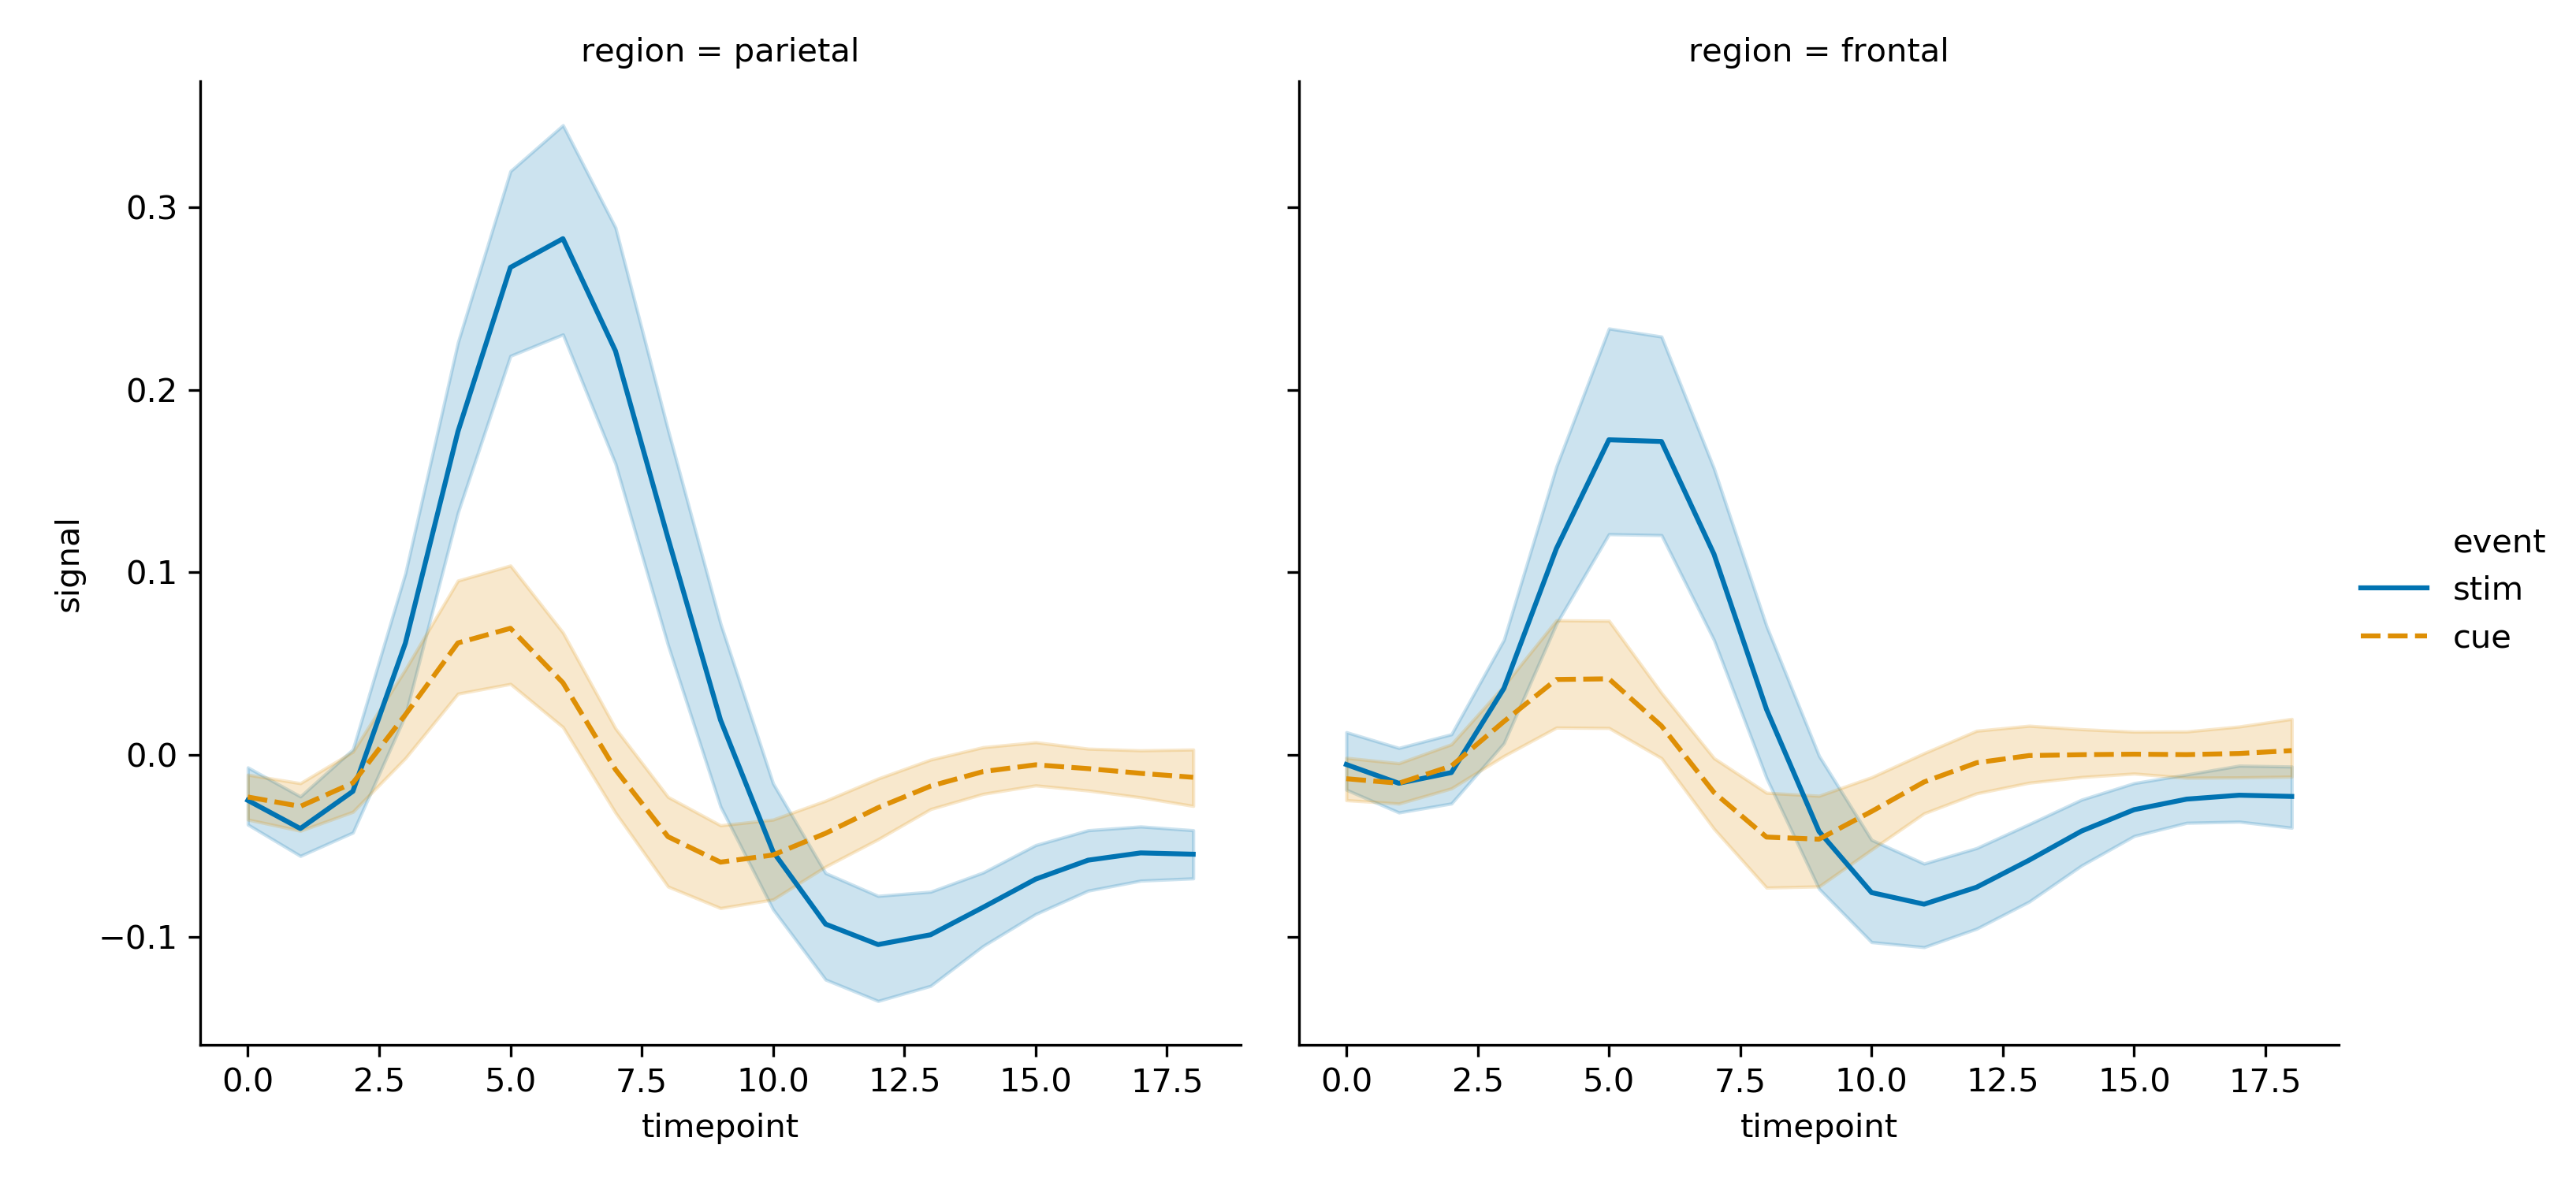
\includegraphics[width = 11cm]{colorblind.png}
    \caption{colorblindness}
    \label{blind}
\end{figure}

\subsection{General culture}
Red stands for tropical zone, yellow stands for temperate zone, blue stands for frigid zone. See Figure \ref{Gculture}.
\begin{figure}[htbp]
    \centering
    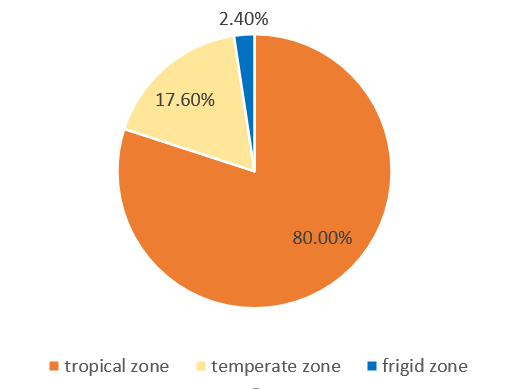
\includegraphics[width = 8cm]{capture.PNG}
    \caption{Biodiversity in different zones on earth}
    \label{Gculture}
\end{figure}


\subsection{Warm color and cold color}
Cold color for new cases (bad news) while warm color for vaccinations(good news). See Figure \ref{color}.
\begin{figure}[htbp]
    \centering
    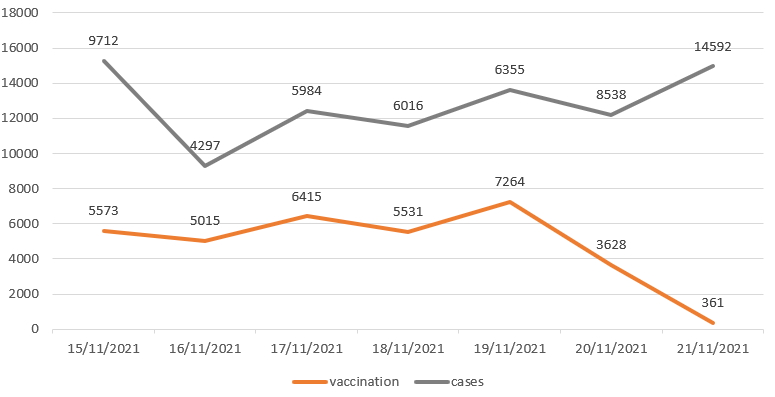
\includegraphics[width = 10cm]{cases.PNG}
    \caption{Covid cases and vaccinations in Switzerland}
    \label{color}
\end{figure}

\subsection{Specific culture}
China stock market uses red color to reflect prices up and green to reflect prices down. See Figure \ref{Sculture}.  
\begin{figure}[htbp]
    \centering
    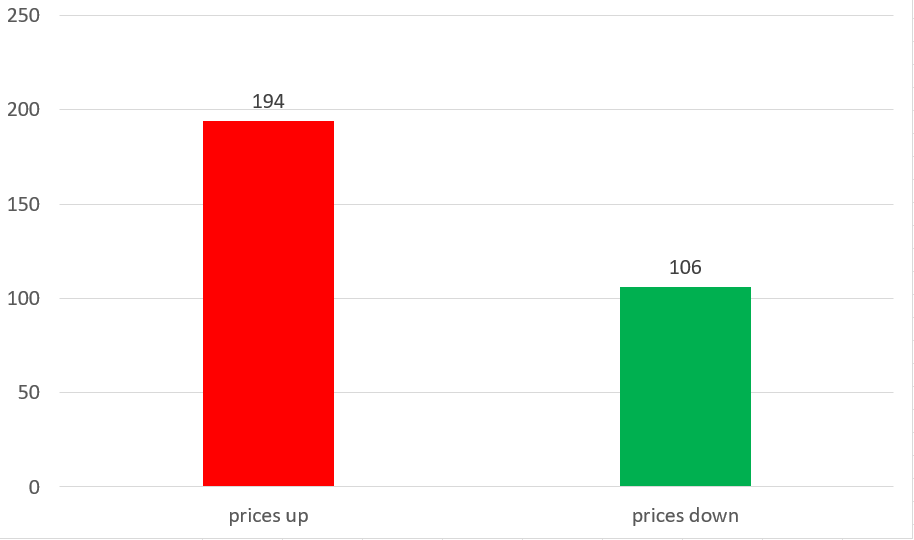
\includegraphics[width = 10cm]{stock.PNG}
    \caption{Prices change of constitute stocks from CSI 300 in 2020}
    \label{Sculture}
\end{figure}

\newpage
\section{Tables}

\subsection{Template}
\begin{table}[htbp]
\centering
\begin{tabular}{|c|c|c|c|}
\hline
Table&title1&title2&title3\\ 
\hline
set1&conten1&conten2&conten3\\ 
\hline 
set2&conten1&conten2&conten3\\ 
\hline 
set3&conten1&conten2&conten3\\
\hline
\end{tabular}
\caption{Table Template}
\end{table}

\subsection{Example of dcolumn}
In order to facilitate observation, we arrange the decimals in the same column of the table by decimal separator alignment. We use LaTeX package dcolumn to implement it.
\begin{table}[htbp]
\centering
\begin{tabular}{c...}
\hline
Weight & \multicolumn{3}{c}{Second-day delivery}                                            \\ \hline
       & \multicolumn{1}{c}{Fedex} & \multicolumn{1}{c}{UPS} & \multicolumn{1}{c}{Airborne} \\
Letter & \$8.00                    & \$6.50                  & \$6.25                       \\
1 lb.  & \$8.00                    & \$7.18                  & \$6.25                       \\
2 lb.  & \$8.79                    & \$8.00                  & \$7.75                       \\
5 lb.  & \$12.14                   & \$10.93                 & \$9.75                       \\
10 lb. & \$18.43                   & \$16.64                 & \$16.00                      \\
50 lb. & \$54.89                   & \$57.11                 & \$58.00                      \\ \hline
\end{tabular}
\caption{List Prices of Express Mail Carriers}
\end{table}


\end{document}